%!TEX root = ../Thesis.tex

\chapter*{General Introduction}
\addcontentsline{toc}{part}{General introduction} % Adds "Introduction" as part-style in ToC
\markboth{Introduction}{General introduction}    % Marks left and right headers as "Introduction"



\section*{1.\, \,  Context of the PhD thesis}

The transportation systems have provided humanity invaluable social and financial benefits, yet they are also intricately linked to adverse outcomes. The widespread use of automobile, while offering convenience, has given rise to challenges such as traffic congestion and an increase in traffic accidents. The investigation of accident causes has been a focal point of rigorous research for many years. According to \cite{humanerrors}, about $85\%$ of accidents can be attributed to human errors. Within this percentage, over $50\%$ are linked to decision errors, wherein drivers receive all relevant environment information but either refrain from making a decision, or choose an incorrect course of action. The remaining $35\%$ is attributed to inattention errors, where drivers are distracted, fail to respond, or lose control of their vehicles. 

A promising avenue to mitigate the majority of human errors is through the automation of the driving tasks. In recent years, the development of fully autonomous vehicles (AVs) for transportation has garnered significant attention from various researchers and industrials globally \cite{duarte2018impact}\cite{rosique2019systematic}\cite{schwarting2018planning}. The fundamental aim of autonomous vehicles is to surpass human perceptions of safety and judgment, particularly in perilous situations, and to produce appropriate actions \cite{dimiathesis}. Driving, being a complex task, demands the autonomous vehicle's ability to make critical decisions, achieved through various intra-vehicle process (e.g., situation awareness and assessment, decision-making, etc.). Moreover, an autonomous vehicle operates within a dynamic driving environment, alongside other road users, adding complexity to the driving task. 


The predominant focus of current autonomous vehicle research revolves around enabling \textit{individual} autonomous vehicles to navigate roads safely. However, there is a growing acknowledgment that to take fully advantage from the benefits of autonomous vehicle technology, certain scenarios will require the \textit{coordination} of relative activities and movements \cite{6949576}. An intriguing area of research is autonomous navigation with a group of vehicles, known as Multi-Vehicle System (MVS). The advantages of MVS span multiple domains, including safety through accident reduction, enhanced passenger comfort promoting health, reduced transportation time by alleviating road congestion, and improved energy efficiency contributing to ecological benefits, among others. Nonetheless, some challenging problems need to be completed to ensure safe coordination between the vehicles in MVS. 



\section*{2.\, \,  Main objectives}

The focus of the research work done in this PhD manuscript corresponds to the subject of MVS coordination ability in what is known in the literature as challenging scenarios \cite{mariani2021coordination}. In other terms, in scenarios such as intersection crossing or on-ramp/off-ramp merging on highway, orchestrating the vehicles' motions becomes a necessity to guarantee the on-road safety. Consequently, the main aim of this PhD work is to study the different topics related to vehicles' motion coordination (i.e. architectures, mechanisms, approaches), to propose a Safe and Energy Efficient Decision/Control Architecture for a Formation of MVS in Dynamic Environment. To accomplish this aim, three main objectives were identified. 




\subsection*{2.1 \, \, Multi-vehicle system for challenging scenarios}

Most current industrial and applied research in the area of autonomous vehicles concerns the methods and tools to enable individual AVs to hit the road safely. However, a number of situations will compulsory require coordinating the relative motions of the AVs to ensure the zero-collision requirement \cite{mariani2021coordination}. For instance, on-ramp merging on highway can be categorized as a challenging where coordination is needed. The highway vehicles evolve in a highly dynamic environment imposed by the highway traffic nature; and conflicting trajectories among the merging vehicles, the vehicles navigating in the secondary on-ramp road, and the highway vehicles are reportedly common \cite{7562449}. 


With the help of the MVS cooperation ability, it is aimed to improve in one hand on-road safety while solving conflicting and unsafe trajectories, and on the other hand, to improve traffic flow by increasing on-road penetration and avoiding bottlenecks (e.g. optimizing the number of vehicles on the merging zone). Undeniably, energy efficiency and passenger comfort are a direct benefit of high flow rate, less idling zones and smooth velocity profiles. 

On-road navigation is not a simple task especially when it has to deal with complex and dynamic scenarios. The first challenge is to take into account the nature of the navigation environment in the definition of the original problem of MVS control, while addressing the complexity of the driving scenario. Coordinating the motion of the vehicles part of the MVS (also known as formation control) is also one full part challenge that needs to be addressed. 


\subsection*{2.2 \, \, Multi-vehicle system navigation in formation}

Safe and reliable formation control method permits to reduce the in-between distance among the MVS, which has a direct consequence on the traffic flow since road capacity is harvested at its best. Vehicles are subject to aerodynamic drag and energy is consumed to face this counter-force. One way to improve the energy consumption is to act on the spacing policy of the formation, in fact, reducing the inter-vehicles distance reduce the aerodynamic drag, consequently energy saving can be part of the benefits of MVS navigation in formation. 

Formation control is also an important part of the traffic management because of its safety and comfort related benefits. In fact, formation control permits to synchronize the motion of the vehicles in order to avoid conflicting trajectories. Long term and short synchronization can be also part of the formation control strategy with the help of formation reconfiguration. Thus, the vehicle motion can be built to impose the minimum vehicle dynamic changes w.r.t. a certain reference dynamic (e.g., minimize the acceleration and the deceleration of the vehicles to travel at a constant speed), what improves the passenger comfort. 


For human driven vehicles, the creation and the navigation in formation is done effortlessly. However, for MVS, the formation control requires a safe and reliable strategy to avoid rear-end collisions, beside the question of the stability that needs to be reliably proven. The first challenge part of the MVS formation control problem is related to formation modeling. Since it is aimed to build a safe and reliable formation control approach, the formation needs to be formulated following mathematical models to facilitate the verification of the formation stability. 

The second challenge behind the formation control approach is through its interactions with the decision-level. A strong connection in-between the formation control approach and the decision-making level needs to be established. The latter helps to ensure that the MVS formation is controlled to track a safe goal, and responds quickly to avoid any risk due to the dynamic nature of the highway environment. 






\subsection*{2.3 \, \,  Cooperative and altruistic multi-criterion decision-making level}





In one hand, it is proposed to take advantage of the navigation in formation part of the MVS paradigm to tackle the coordination maneuver related to the on-ramp merging on highway scenario. In the other hand, MVS technology is harnessed to capitalize on its benefits, including improved safety, enhanced passenger comfort, and optimized energy efficiency. 


However, effective MVS navigation requires support of a suitable decision-making level. Fundamentally, the primary responsibility of the decision-making level is to define the formation goal, and ensuring the safety and feasibility of this goal falls within its purview. 

In the context of the targeted decision/control architecture, the decision-making level's task goes beyond merely selecting a safe and feasible formation goal. Since the aim is to fully exploit the MVS capabilities, the first challenge in decision-making is how to incorporate the following decision criteria: (a) safety, (b) passenger comfort, and (c) energy efficiency. These three criteria must be seamlessly integrated into the decision-making level, with their respective contributions meticulously balanced. 


An MVS comprises multiple vehicles that decide to navigate together for a specific duration. In this PhD thesis, the MVS vehicles are supposed to be altruistic. In other terms, under the cooperation paradigm, the vehicles accept to participate by making reasonable efforts such as the MVS performs the merging maneuver. Consequently, while the MVS has its overarching global goal, each vehicle within the MVS has its individual goal. For example, in the case of on-ramp merging on highway performed by an MVS, the MVS goal is to execute the merging maneuver without causing accidents within the merging zone. However, the individual goals of the vehicles may differ, depending on their roles as highway or merging vehicles. Thus, the second goal of the decision-making level is to select the formation goal, for instance performing the MVS merging maneuver safely, while ensuring the MVS performance efficiency (e.g., passenger comfort, energy efficiency). In addition of taking into account the individual contributions of each vehicle within the MVS toward its global goal, and avoiding the selection of unfair goals with respect to the vehicles' participation. 




\section*{3.\, \,  Manuscript outlines and contributions}
According to the above mentioned PhD context and objectives, the ultimate goal of this PhD thesis is to propose a safe and energy efficient decision/control architecture for a formation of MVS in dynamic environment. The dedicated endeavor to achieve  this goal is transcribed in this manuscript, which is comprehensibly divided into two parts. The outline of the PhD manuscript is depicted in Figure 1. More precisely, the first part, which contains two chapters, targets to discuss the state of the art - in particular the current research gap for autonomous vehicles cooperative motion planning and decision-making for MVS in a complex dynamic environment such as on-ramp merging on highway - as follows: 

\begin{itemize}
    \item \textbf{Chapter 1 - From individual automated vehicle to multi-vehicle system}\\
     Given that the MVS is composed of multiple AVs, this chapter initiates with a concise overview of the AV technology; laying the groundwork of the subsequent discussion on MVS. It then delves into the central focus of this chapter, namely, the MVS paradigm. Following the presentation of the key concepts related to the MVS, this chapter explores projects in which MVS is actively engaged. These projects serve as examples of technological advancements and innovations aimed at enhancing the MVS capabilities when navigating in on-road environments. Furthermore, the chapter delves into the cooperative navigation of MVS, examining scenarios from a comprehensive perspective. 

     \item \textbf{Chapter 2 - Cooperative motion planning and decision-making for MVS: architecture overview}\\
       This chapter aims to offer a detailed exploration of the MVS control architecture by delving into its modules and different processes. Furthermore, it provides insights into paradigms utilized in the construction of the MVS control architecture. Since formation control plays a crucial role in the aimed decision/control architecture, the chapter reviews and discusses various formation control approaches. Finally, it presents a literature overview, emphasizing MVS applications within complex environments. An evaluation through the prism of traffic throughput, energy efficiency and negotiation is proposed. 
    

    
\end{itemize}

\begin{figure}[!h] \label{fig:outlines}
        \centering 
        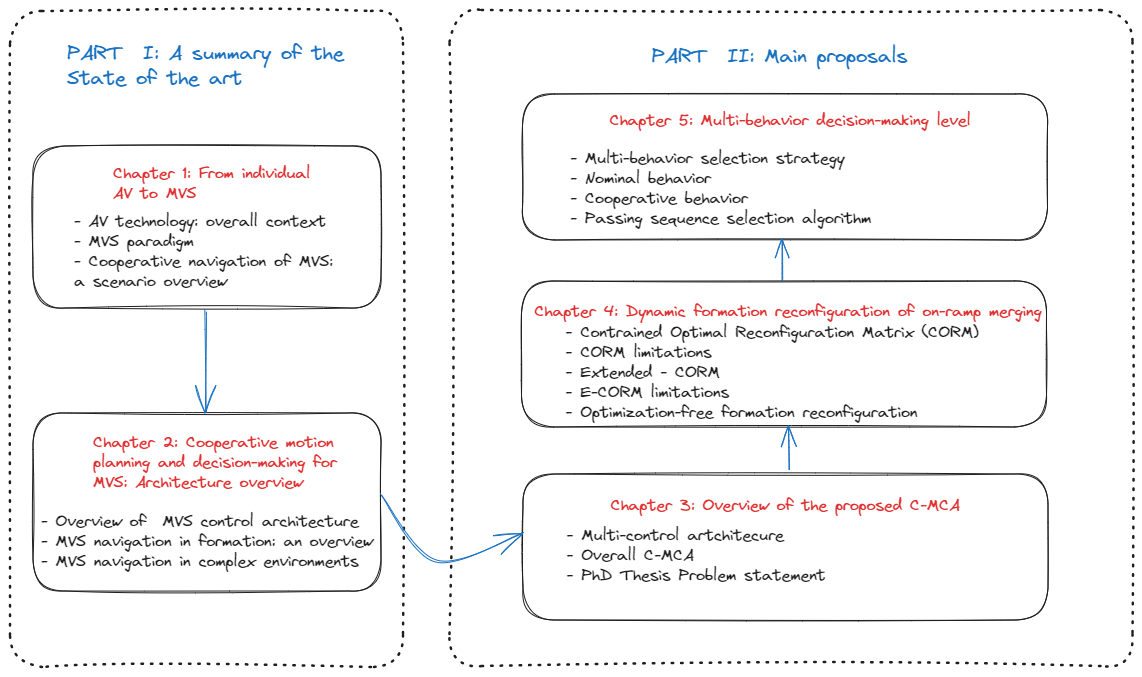
\includegraphics[width=13cm,height=18cm,keepaspectratio]{chapters/outlines}
       % \vspace{-2.3mm}
        % \begin{center}
        \textsc{Figure 1:} The outline of the PhD manuscript
         %\end{center}
        %\caption{The outline of the PhD manuscript}
        \end{figure}


The last part of the PhD manuscript concentrates on the primary approaches and proposals addressed in this dissertation, which can be categorized into three chapters (cf. Figure 1): 

\begin{itemize}
    \item \textbf{Chapter 3 - Overview of the proposed Cooperative multi-controller architecture}\\
     The central theme of this chapter revolves around the introduction and exploration of the proposed Cooperative Multi-Controller Architecture (C-MCA). It starts with a concise overview of the background of multi-controller architecture to establish the context for delving into the intricacies of the proposed C-MCA. The chapter extensively discuss the various modules within the C-MCA, with a particular emphasis on the decision-making and planning levels, as these are pivotal in accomplishing the goals outlines on the decision/control architecture. In addition to the foundational information related to the PhD thesis problem statement. 










    \item \textbf{Chapter 4 - Dynamic formation reconfiguration of on- 
     ramp merging }\\
     The chapter initiates with an introduction of the Constrained Optimal Reconfiguration matrix (CORM) algorithm, a key element for formation control, accompanied by pertinent simulation results. 
    
     Than the chapter focuses on  providing an in-depth exploration of the Extended - Constrained Optimal Reconfiguration Matrix (E-CORM). It initiates with a concise overview of the limitations associated with the CORM, the chapter focuses on the enhancements made to overcome these limitations through the introduction of the E-CORM. The algorithm associated with the E-CORM is elucidated, and subsequent attention is given to the presentation of the simulation results. 

     The latter part of the chapter is dedicated to evaluating the limitations of both the CORM and the E-CORM to devise a suitable formation reconfiguration strategy. Within this context, a novel optimization-free formation reconfiguration strategy, named Formation Reconfiguration Approach base on an Online Control Strategy (FRA-OCS), drawing inspiration from both the CORM and the E-CORM, is introduced in details. The chapter culminates with the presentation of simulation results for this newly proposed formation reconfiguration strategy. 









    
        \item \textbf{Chapter 5 - Multi-behavior decision-making level}\\
This chapter is specifically focused on elucidating the intricacies of the decision-making level within the proposed C-MCA for MVS engaged on on-ramp merging on highways. The multi-behavior selection strategy, an integral part of the decision-making level, is expounded upon through the comprehensive presentation of the developed behaviors. Additionally, the chapter delves into the bi-directional link between the decision-making level and the formation control level, providing detailed insights into the selection of the passing order of the vehicles in the merging zone. The effectiveness of the proposed multi-behavior decision-making level is evaluated through the presentation of various simulation results.  

\end{itemize}


General conclusions are summarized at the end of the manuscript, additionally,  it outlines potential avenues for future research related to this PhD thesis. 